\chapter{Proposed Solution}

In this chapter we define in detail the solutions proposed by this thesis. The main goal is performing doors detection by autonomous agent.

\section{Work Overview}
\label{sec:solution}
In this thesis, we face the problem of doors detection in autonomous mobile robots. In the following paragraphs, we expose the proposed solutions about the three main problems this work addresses: how to build of the doors detector, how to improve the module's performance, and how to compose and evaluate a visual dataset in a Robotic Vision application.

\paragraph{Build the Doors Detector Module} At first, we reduce to problem of finding doors in indoor environments to a well-known Computer Vision task: object detection in RGB images. After a literature review about this subject, we propose a module to detect doors based on DETR (DEtection TRanformer) \cite{detr}, a deep end-to-end architecture that performs object detection exploiting the Transformers' power \cite{transformer}. DETR views object detection as direct set prediction problem, removing the need for many hand-designed components (like a non-maximum suppression or anchor generation) that explicitly encode prior knowledge about the task. Thanks to the novel Transformer's architecture, DETR extract features from the image and then finds the pair-wire relations between them. In this way, it reasons about the entire image as context. The authors demonstrates that DETR accuracy and run-time performance are comparable the well-established and highly-optimized Faster R-CNN baseline \cite{fasterrcnn} on the challenging COCO object detection dataset \cite{coco}. Despite this, DETR is an enormous networks with tens of millions of parameters and it is extremely data hungry: the authors train DETR for 300 epoch with COCO's examples randomly modified with data augmentation procedures (e.g. resize, crop, scale, etc.). This thesis demonstrates the versatility of DETR with respect to other object detection task, even with smaller dataset than COCO.

\paragraph{Increase the Detector's Performance} Another goal of this thesis is to improve the doors detector's accuracy. To address this problem, we do not focus on the deep module that performs object detection, but we reason about its context of use. We focus on an typical deployment scenario for indoor mobile robots (as described in Sec. \ref{sec:deploymentscenario}). We argue that, often, a robot is deployed in a single environment and works inside it for a log time. Furthermore, thanks to  the wayfinding principles described in Sec. \ref{sec:goals}, an indoor scenes presents the a coherent visual aspect. This is also true for doors: a single environment presents a few types of doors that are repeated in multiple locations. The method to increase the doors detector's accuracy exploits these intuitions. Our approach aims to specialize the model for working in a precise environment using the fine-tune technique. Fine-tuning on pre-trained ImageNet classification models \cite{verydeepimagenet, resnet} has achieved impressive results for tasks such as object detection \cite{fasterrcnn, yolo, yolov2} and is becoming the common way for solving computer vision problems. Fine-tuning is a simple and effective
approach of transfer learning: it concerns on training a deep model with common large datasets (such as ImageNet \cite{imagenet} or Microsoft COCO \cite{coco}). Then, the pre-trained model is re-trained with a few new data to solve a more refined task. In this way, the network's weights are set using a source dataset with a large number of examples providing a better
model initialization for a target task than random initialization. This is useful to speed up the training, overcome small dataset size, or prevent overfitting. We use the same principle to increase the performance of the proposed doors detector. Initially, DETR is trained with a general doors dataset that contains examples from multiple environments. After that, to emulate the ideal deployment scenario in which a robot operates in an unknown environment not included in the training phase, DETR is fine-tuned using a little set of new unseen data acquired directly form the new scene. In this way, the general door detector, built in the development phase, specializes itself using new examples for working in a precise environment, thus increasing its accuracy. We also investigates the quantity of new data necessary to obtain a significant performance improvement.

\paragraph{Compose and Evaluate the Visual Dataset}
This thesis address a Robotic Vision task that completely differs from Computer Vision application. As reported in \cite{surveydeeplimits}, perception is only one part of a more complex, embodied, active, and goal-driven system in robotics.
In a simplified view, whereas Computer Vision takes images and translates them into information, Robotic Vision translates images into actions. Furthermore, an autonomous agents operates in open-set conditions. A module used by a robot can assign high-confidence scores to unknown objects or falsely recognize them as one of the known classes. In order to understand how the doors detector performs in different environments, this thesis proposes a method to acquire a dataset of RGB images trough simulation. We collect both positive images (that contains doors to detect) and negative frames (that do not depict objects of interest) from multiple scenes. We use Gibson \cite{gibson} to simulate an agent and its visual perception in environments taken from Matterport3D worlds dataset \cite{matterport}. A mobile robot navigates in an environment following an exploration strategy, avoiding going too close to walls, furniture, and obstacles in general. Furthermore, a robot percept the environment from different point of views, according to its position in the scene and the height of the camera. To take this fact into account, we propose an approach to select the different locations from which to acquire the data. This method, based on the work presented by \citeauthor{segmentationsurvey} \cite{segmentationsurvey}, computes the Voronoi Graph of the occupancy grid maps of an environment. The locations form which acquire the RGB images are chosen by sub-sampling the Voronoi Graph with a distance value. Thank to this algorithm, the doors dataset is acquired simulating a possible exploration strategy, avoiding to acquire wrong or noise images that can degrade the model accuracy.


\section{Doors Detector}

The main goal of this thesis is to propose a doors detector that is able both to find doors within RGB images and understand their status (open or closed). We reduce these problems to a precise Computer Vision's task: object detection. The doors detector we propose is built with DETR \cite{detr}, a novel end-to-end deep module based on Tranformers. Before talking about DETR and how it is used to detect doors, we review the most relevant aspects in the theory of Deep Learning.

\subsection{Deep Learning Review}

Deep Learning is a sub-field of Machine Learning, that is the study of computer algorithms that can improve automatically through experience and by the use of data. We define some important aspect of Machine Learning before talking about the proposed approach to detect doors. Machine Learning is a powerful technique suitable when it is not feasible to develop a standard algorithm to solve a difficult task. A \textit{learning algorithm} uses sample pairs of training data to create a model, also called predictor, that is able to classify other unseen data. The first important aspect for a machine learning problem is the dataset. Typically, a dataset is composed by pairs of data taken from two different sets: the \textit{data domain} and the \textit{label set}.

\begin{definition}[Data domain]
	We use $X$ to denote the set of all possible data points for a given learning problem. Each data point is composed by features. In some cases, the features are encoded as vectors of real numbers. Such a vector representation is \textit{natural} whenever the data consist of homogeneous quantities, like pixels in an image or words' frequencies in a document. A data point is denoted as $x \in X$ and it is defined as a vector of feature $x = (x_1, ..., x_d)$.
\end{definition}

\begin{definition}[Label set]
	We use $Y$ to denote the set of all possible labels for a data point of a given learning algorithm. For a classification problem, the label set is typically finite and small (such as $Y = \{sport, policies, business\}$ for a documents categorization task).
\end{definition}

In a \textit{supervised} learning problem, the data point are tagged with their respective ground truth labels. In particular, the dataset's entries are pairs $p = (x, y)$, where $x \in X$ is a data point and $y \in Y$ is the label assigned to it. A \textit{supervised} learning algorithm is a technique that aims to build a model learned from a \textit{training set}. This paradigm is called \textit{learning by examples}. An example is a pair $p=(x, y)$ (where $x$ is a data point represented by a feature vector and $y$ is its ground truth label) and the training set is composed by a series of examples $S=\{(x_1, y_1), ..., (x_m, y_m)\}$. A \textit{supervised learning algorithm} for \textit{learning by examples} receives a training set and outputs a learned model.

\begin{definition}[Model]
	A model is a function $f:X \to Y$ that maps data points to labels.
\end{definition}

The training examples come from some generally unknown probability distribution and the goal of a learning problem is to infer a function that approximates this distribution (or makes a generalization of it) to produce sufficiently accurate predictions in new cases. In order to estimate the predictive power of a model, we typically use a \textit{test set}. This is a set of examples $T=\{(x_1', y_1'), ..., (x_n', y_n')\}$ that the learning algorithm does not have access during the training phase. Each pair in the \textit{test set} are fed into the model in order to measure the goodness of each prediction compared with the ground truth label. This measure is computer using the \textit{loss function}.

\begin{definition}[Loss function]
	A loss function $\ell(y, \hat y)$ measure the discrepancy between the predicted label $\hat y$ and the ground truth label $y$. For a correct prediction, $\ell (y, \hat y) = 0$.
\end{definition}

A way to train a learning model is the Empirical Risk Minimization (ERM) approach. The test set allows to determine the predictive power of a learned model on unseen new data. To measure the goodness of a predictor, we can calculate the \textit{test error} over a test set $S$. 

Given a loss function $\ell$, the test error is
\begin{equation}
\frac{1}{n} \sum_{t=1}^{n}\ell(y_t', f(x_t'))
\end{equation}
where the $n$ is the test set's cardinality ($n = |S|$), $y_t'$ is the ground truth label of the f-th test example and $f(x_t')$ returns the predicted label from the t-th data point. Since the test set is disjoint from the training set, ERM offers a theory to design learning algorithms that generate predictors with a low test error considering only the training set. ERM assumes that the \textit{training error} (the error computed over a training set $T$) of a predictor is directly correlated to its test error. The training error is given by 

\begin{equation}
\hat \ell(f) = \frac{1}{m} \sum_{t=1}^{m}\ell(y_t, f(x_t))
\end{equation}
where the $m$ is the test set's cardinality ($m = |T|$).



\begin{definition}[Empirical risk minimization] 
	Let $\mathcal{F}$ a set of predictors and $\ell$ a loss function. The empirical risk minimizer (ERM) is the learning algorithm that outputs some predictor in $\mathcal{F}$ minimizing the training error
	
	\begin{equation}
	\hat f \in \argmin_{f \in \mathcal{F}} \hat \ell(f).
	\end{equation}
	The notation $\in$ denotes there could be multiple $f \in \mathcal{F}$ that minimizing the training error.
\end{definition}

The ERM algorithm fails when no predictors in $\mathcal{F}$ have a low test error, in particular when 

\begin{equation}
	\min_{f \in \mathcal{F}} \frac{1}{n} \sum_{t = 1}^{n} \ell(y_t', f(x_t'))
\end{equation} 
is high. The two main ways of failing for a generic learning algorithm are:
\begin{itemize}
	\item \textbf{underfitting:} when a learning algorithm tends to outputs predictors whose test and training errors are high and closed to each other. This situation could depend on the training test size: if it is too small it can not represents well the data points' distribution or $\mathcal{F}$ (the set of the possible predictors) are too large with respect the training set dimensions. Another reason that causes underfitting is the cardinality of $\mathcal{F}$. If the set of the possible predictors is small, there could not be a subset of them with small test error. This means that the learning algorithm is not complex enough to output good learned models. In other words, when a model underfits it is not able to generalize well the problem, failing to classify example from both training and test sets;
	\item \textbf{overfitting:} when a learning algorithm tends to output predictors whose training error is low (or it tends to zero) and test error is high. In this situation, the predictors produced by a learning algorithm learn too much from the training data and, as a result, are unable to produce good predictions on new data. This means that those predictors do not generalize the problem, but are specialized in dealing only with the data using during the training phase.
\end{itemize}

When $A$ is a ERM learning algorithm and the size $m$ of the training set is fixed, we should expect overfitting when $\log_2|\mathcal{F}| \gg m$, so the set of possible predictors is to large with respect to the training set's size. On the other hand, when $\log_2|\mathcal{F}| \ll m$ we should expect underfitting.

Deep Learning is a subfield of Machine Learning based on \textit{neural networks}. This learning algorithm is inspired by the information processing and distributed communication of biological brains. Neural networks (NNs) are a large and complex class of predictors, based on artificial neurons.

\begin{definition}[Neuron]
	An artificial neuron is a mathematical function inspired from biological neuron and it represents the elementary units in an artificial NN. The matematical function implemented by a neuron is $g(x) = \sigma(\omega^\intercal \cdot x)$, where $\sigma$ is the activation function, $\omega$ is the weight vector of learnable parameters,and $x$ is the input vector of the neuron. This means that each input is separately weighted and the sum is passed through a non-linear function. The activation function usually have a sigmoid shape and often it is monotonically increasing, continuous, and bounded. 	
\end{definition}

Artificial neural network are composed by a series of simple predictions made by neurons. The adjective ``deep'' in Deep Learning refers to the use of multiple layers in NNs. The most simple model of neural network is feedforward NN. 

\begin{definition}[Feedforward neural network]
A feed forward neural network computes functions of the from $f : \R^d \to \R^n$. Its structure is a directed acyclic graph $G = (V, E)$, in which $V$ is the set of nodes (neurons) and $E$ is the set od edges that connects the neurons. The vertices in $V$ are divided into three subgroups: $V = V_{in} \cup V_{hid} \cup V_{out}$, where $V_{in}$ (with $|V_{in}| = d$, the feature space's dimension) are the input nodes which have no incoming edges, $V_{out}$ (with $|V_{out}| = n$, the number of labels) are the output nodes which have no outgoing edge, and $V_{hid}$ are the hidden nodes, which have both incoming and outgoing edges.
\end{definition}

The most simple form of feedforward neural network is the multi layered perceptron (MLP), in which the nodes of $V$ can be partitioned in a sequence of layers such that each node of a layer has incoming edges only from
nodes in the previous layer and outgoing edges only to nodes of the next layer.  The layers containing the hidden nodes are called hidden layers. 

\begin{figure}[h!]
	\centering
	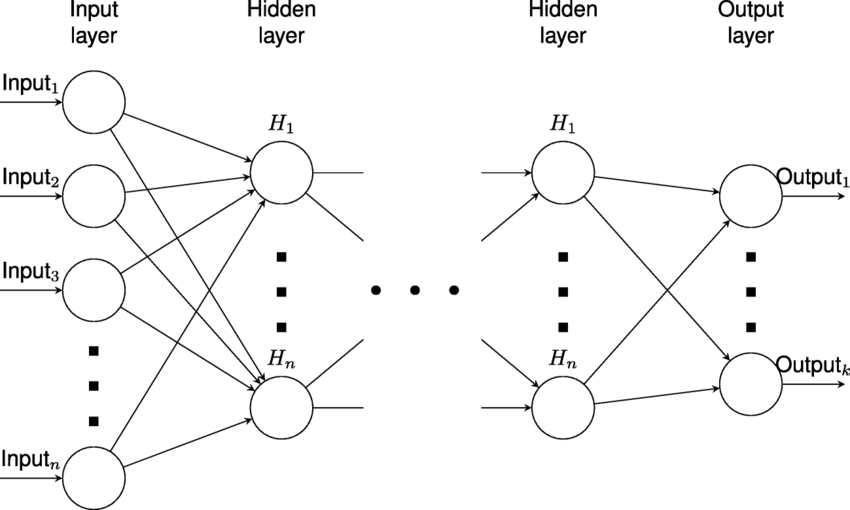
\includegraphics[width=0.9\linewidth]{images/mlp.png}
	\caption{An example of feedforward neural network, with $d$ input nodes and $n$ output nodes. In this example, the connectivity between layers is complete (there are no missing edges).}
\end{figure}

The learnable parameters are the weights assigned to the edges between neurons. 
A parameter $\omega_{i,j} \in \R$ (called weight) is associated with every edge pair $(i, j) \in E$.  We use $W$ to denote the $|V | \times |V |$ weight matrix, where $(i, j) \notin E$ implies $\omega_{i,j} = 0$. The graph $G$, the weights matrix
$W$, and the activation function $\sigma$ define the function $f = f_{G,W,\sigma}$ computed by the network.  Note that when $n = 1$ (one output node) and $|V_{hid}| = 0$ (no hidden nodes), then $F_{G,\sign}$ only contains linear classifiers of the form $f(x) = \sign(\omega^\intercal \cdot x)$. The training of neural networks is not trivial. The most natural approach for training a model in $\mathcal{F}_{G,\sigma}$ is ERM.
Unfortunately, this method could not efficiently applied to neural networks. 

\begin{theorem}
	For every integer $k \geq 3$, let $G$ be a network with $d$ input nodes, a single hidden layer containing $k + 1$ nodes (one of which has constant value 1), and a single output node. Then the problem of minimizing the zero-one loss training error in $\mathcal{F}_{G,\sign}$ is NP-hard. 
\end{theorem}

The models considered by this theorem are simplified neural networks to solve a \textit{binary classification} task using the zero-one loss (equation \ref{formula:zero-oneloss}) with a single hidden layer composed by four or more neurons. 

\begin{equation}
	\label{formula:zero-oneloss}
	\ell(y, \hat y) = 
	\begin{cases}
	0 & \text{if $y = \hat y$} \\
	1 & \text{if $y \neq \hat y$}
	\end{cases}
\end{equation}

This theorem demonstrates the inefficiency of ERM for a simple NN. This means that this theorem is true even for more complex neural networks and different tasks. ERM remains NP-hard even when $\mathcal{F}_{G,\sign}$ contains only linear classifiers (i.e., $G$ has no hidden nodes). However, while the cause of NP-hardness in linear models was the non-convexity of the loss function (zero-one loss in this case), in multi-layered neural networks the problem is inherent to their structure. The key observation is that the presence of hidden nodes in NN makes the loss function $\ell_t$ over a example $(x_t, t_t)$ non-convex in the weights matrix $W$ even when $\ell(x, y)$ is convex for all $y$. In general, the problem of minimizing a non-convex function is computationally intractable.  

This is because NNs are successfully trained using algorithms that reduce the training error without any mathematical guarantee on the solution's quality. The training procedure starts with a forward propagation of the training examples in the neural network. After that, the outputs are used to quantify how good the predictions are and the error are back-propagated in the network using a descent algorithm. The standard training algorithm for NNs is stochastic gradient descent (SGD):

\begin{equation}
\omega_{i, j} \leftarrow \omega_{i, j} - \eta_t \frac{\partial\ell_{Z_t}(W)}{\partial\omega_{i, j}} \quad \quad (i, j) \in E,
\end{equation}
where $Z_t$ is the index of a random training example and $\eta$ is an hyper-parameter that controls the step size (also called learning rate). The main idea is to calculate the partial derivative of the loss function, calculated on a training data point $t$ and the current NN status (described by the weights matrix $W$), over all the learnable parameters to adjust their values. In order to speed up convergence, the training samples can be grouped in mini-batches. Because the training error is a non-convex function of $W$, the SGD algorithm essentially finds only local minima of the training error. The procedure to perform gradient descent on feedforward NNs is known as \textit{error back-propagation}. 

\subsection{DETR}

The doors detector proposed by this thesis is based on DETR \cite{detr} (DEtection TRansformer), a novel deep approach to perform object detection. In DETR, object detection problem is modeled as a direct \textit{set prediction}, making the detection pipeline a simple end-to-end unified architecture. Modern detectors address this set prediction in an indirect way using hand crafted algorithms based on a large set of proposals \cite{yolo} or anchors \cite{focalloss}. Their performances are significantly influenced by these post-processing steps to collapse near-duplicate predictions, like non-maximum suppression or anchor generation. The first important aspect the architecture (explained in Sec. \ref{sec:detrarchitecture}). DETR uses a Transformer to finds complex relationships between features extracted in the same image. In this way, the model reasons about the whole image context without considering any form of prior knowledge about the task. The second important aspect to address the set prediction problem are the loss functions (described in \ref{sec:detrlosses}). DETR uses a set loss function which performs bipartite matching between predicted and ground-truth objects.

\subsubsection{DETR Architecture}
\label{sec:detrarchitecture}
The architecture of DETR (reported in Fig. \ref{fig:detrarchiecture}) consists on three main components: a convolutional neural network (CNN) backbone for features extraction, an encode-decoder transformer to capture the relationships between the extracted features, and a simple feed forward network (FFN) that makes the final detection prediction (the coordinates of the bounding boxes and their relative labels).

\begin{figure}[h!]
	\centering
	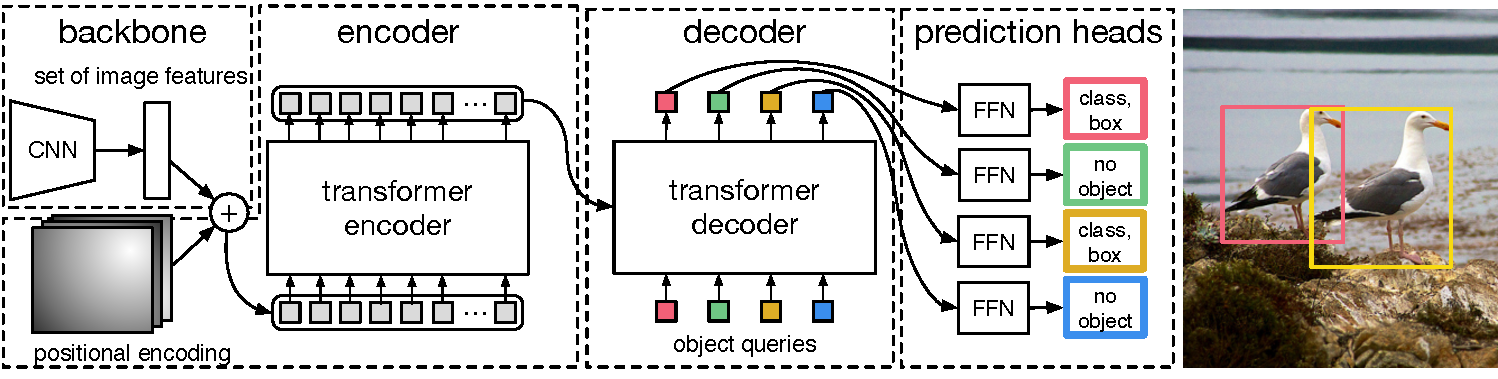
\includegraphics[width=\linewidth]{images/detrarchitecture.pdf}
	\caption{The architecture of DETR. It uses a conventional CNN backbone to learn a 2D representation of an input image. Then, this representation is flattened and encoded before being passed into the transformer encoder. The transformer decoder then takes as input a small fixed number of learned positional embeddings, called \textit{object queries}, and additionally attends to the encoder output. Finally, each output embedding of the decoder is processed by a  feed forward network (FFN) that predicts either a detection (class and bounding box) or a ``no object'' class. Image from \cite{detr}.}
	\label{fig:detrarchiecture}
\end{figure}

\paragraph{CNN Backbone} The first element in DETR's architecture is a CNN backbone.  Ideally, any backbone can be used depending upon the complexity of the task to provide low dimensional representation of the image extracting features from it. Starting from the initial image $x_{img} = \R^{3\times H_0\times W_0}$ (with 3 color channel and dimension $H_0$, $W_0$), a conventional CNN backbone generates a lower-resolution activation map $f \in \R^{C×H×W}$. Typical values used in this paper are $C = 2048$ and $H, W = \frac{H_0}{32}, \frac{W_0}{32}$. 

The authors uses ResNet (residual network) \cite{resnet} as CNN backbone, a neural network that solve the issue of vanishing gradient. This problem makes deeper neural network more difficult to train and optimize: when network depth increasing, accuracy gets saturated and then degrades rapidly. This unwanted situation is called \textit{degradation} (of training accuracy). Unexpectedly, such degradation is not caused by overfitting, and adding
more layers to a deep model leads to higher training error. The authors address the degradation problem by introducing a \textit{deep residual learning} framework, commonly called ResNet. The proposed method is based on the insight that a few overlapping layers can fit a residual mapping instead of directly fitting a desired underlying mapping. This principle is formalized as follow. Let $\mathcal{H}(x)$ be the desired underlying mapping fit by a few stacked layers (not necessarily the entire net), where $x$ denotes the inputs of the first layer. Since multiple non-linear layers can approximate  non-linear functions, then  the same layers can approximate the residual functions $\mathcal{H}(x) - x$. The authors let these layers approximate a residual function
$\mathcal{F}(x) := \mathcal{H}(x) - x$:  now the original function becomes
$\mathcal{F}(x)+x$. The authors hypothesize that it is easier to optimize the residual mapping than to optimize the original, unreferenced mapping.  If the optimal function is closer to an identity
mapping than to a zero mapping, it should be easier for the
solver to find the perturbations with reference to an identity
mapping, than to learn the function as a new one. This means that subsequent blocks in our network are thus responsible for fine-tuning the output of a previous block, instead of having to generate the desired output from scratch.

\begin{figure}[h!]
	\centering
	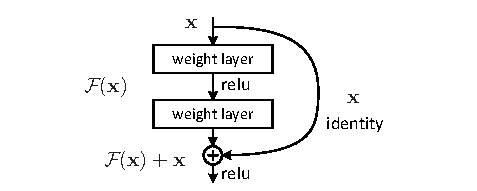
\includegraphics[width=0.9\linewidth]{images/residualblock.pdf}
	\caption{Residual learning: a building block. The formulation of $\mathcal{F}(x)+x$ can be realized with a ``shortcut connection'', that skips one or more layers. Image from \cite{resnet}.}
	\label{fig:resblock}
\end{figure}

\paragraph{Transformer Encoder-Decoder} The second part of DETR is a Transformer \cite{transformer}, a novel sequence-to-sequence (Seq2Seq) architecture that transforms a given sequence of elements, such as the sequence of words in a sentence, into another sequence. Seq2Seq models are particularly useful for natual language process tasks (NLP), text classification, machine translation and
question answering. Among their salient benefits, Transformers enable modeling long dependencies between input sequence elements, support parallel processing, and require minimal inductive biases for their design. Recent studies \cite{surveytransformer} demonstrates the application of Transformer in Computer Vision. By using a Transformer model, DETR globally reasons about all objects together using pair-wise relations between them and being able to use the whole image as context. In this way, DETR predicts (in a single pass) a set of objects and
models their relations. Since DETR performs object detection, the sequence of words in a sentence is replaced with a sequence of feature extracted from an image.

Tranformer model, proposed by \citeauthor{transformer} \cite{transformer}, is the first transduction model relying entirely on self-attention mechanism to compute representations of its input and output without using RNNs or convolutions. Self-attention, sometimes called intra-attention, is an attention mechanism that relates different positions
of a single element in a sequence to compute a representation of the entire sequence. In other words, the attention mechanism decides at each step which parts of the sequence are important by assigning a weight to each element. The Transformer architecture (Fig. \ref{fig:transformerarc}) is based on a encoder-decoder structure. In a general way, the encoder maps an input sequence of symbol representations $(x_1, ..., x_n)$ into a sequence of continuous representations $z = (z_1, ..., z_n)$. Given $z$, the decoder then generates an output sequence $(y_1, ..., y_m)$ of symbols one element at a time. 

\begin{figure}[h!]
	\centering
	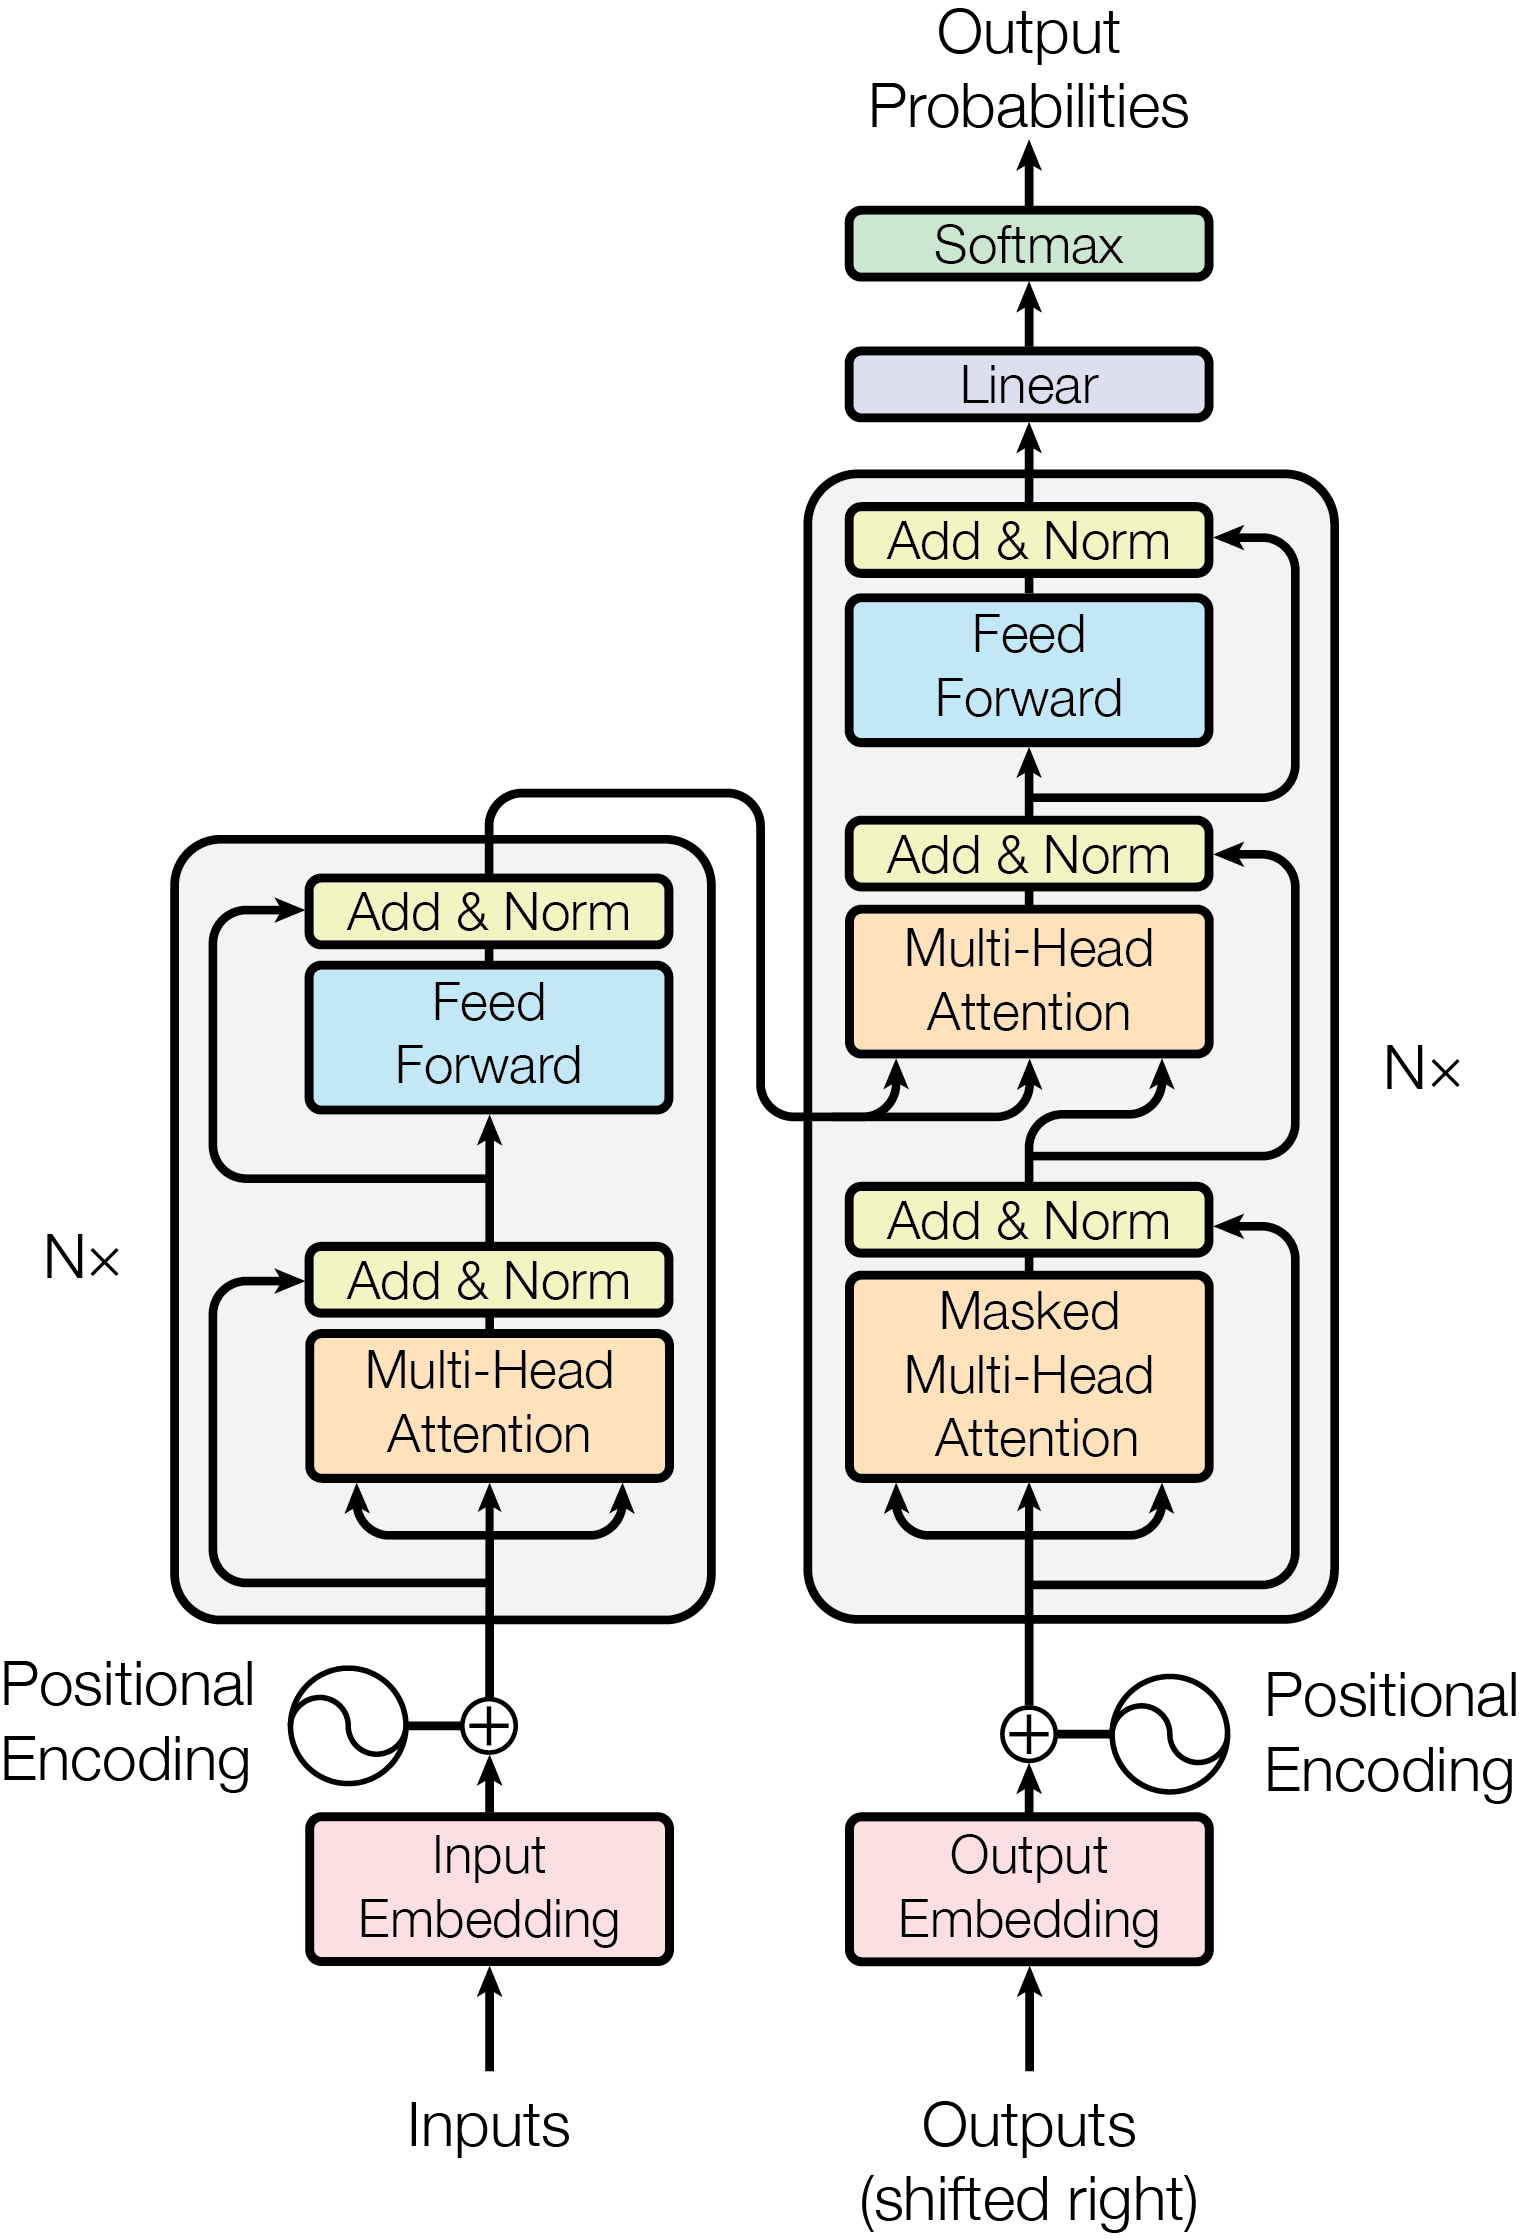
\includegraphics[width=0.7\linewidth]{images/transformerarchitecture.png}
	\caption{The Transformer model architecture. Image from \cite{transformer}.}
	\label{fig:transformerarc}
\end{figure}

More specifically, the Transformer's encoder  is composed of a stack of $N = 6$ identical layers. Each layer has two sub-layers: the first is a multi-head self-attention mechanism, and the second is a simple, position-wise fully connected feed-forward network. The authors added a residual connection (like ResNet \cite{resnet}) around each sub-layer, followed by layer normalization. The output of each sub-layer is $\text{LayerNorm}(x + \text{Sublayer(x)})$. The decoder is also composed of a stack of $N = 6$ identical layers. Each of them has the same sub-layers of the encoder with a third one which performs multi-head attention over the output of the encoder stack. The authors modify the self-attention
sub-layer in the decoder to prevent positions from attending to subsequent positions. This masking, combined with fact that the output embeddings are offset by one position, ensures that the predictions for position $i$ can depend only on the known outputs at positions less than $i$.

DETR \cite{detr} uses a standard Transformer developed for natural language process as proposed in \cite{transformer}. The high-level activation map $f$ extracted form the CNN backbone is rescaled form $C$ to a smaller dimension $d$ by a $1\times1$ convolution. The new feature map fed into the Transformer's encoder is $z_0 \in \R^{d, H, W}$. Since the encoder expects a sequence as input, the feature map $z_0$ is collapsed the spatial into one dimension, resulting in a $d\times HW$ feature map. The decoder transforms $N$ embeddings of size $d$.  The difference with the original Transformer \cite{transformer} is that DETR decodes the $N$ objects in parallel at each decoder layer. These input embeddings (called \textit{object queries}) are positional encoding vectors learned by the model during the training phase. They are passed to the input of each attention layer. Since the decoder is permutation-invariant, the $N$ input embeddings must be different to produce different results. Each object queries is transformed into an output embedding by the decoder. The number of object queries is an hyper-parameter and it must be greater that the quantity of different objects in an image.

\paragraph{Feed-Forward Networks} The $N$ object queries produced by the decoder are  independently classified into box coordinates and class labels by
a feed forward network, resulting $N$ final object predictions. The final predictor is composed by a 3-layer perceptron and a linear projection layer. The perceptron predicts the normalized center coordinates, height and width of the bounding boxes while the linear layer predicts the class labels. Since DETR predicts a
fixed-size set of $N$ bounding boxes, where $N$ is much larger than the
actual number of objects of interest in an image, an additional special class label $\varnothing$ is used to represent that no object is detected within a slot (it indicates the ``background'' class).

\subsubsection{DETR Loss Functions}
\label{sec:detrlosses}

DETR \cite{detr} simplifies the detection pipeline by dropping multiple hand-designed components that encode prior knowledge, like spatial anchors or non-maximal suppression. To address set prediction in a fully end-to-end way, DETR uses a novel loss function, called \textit{object detection set prediction loss}, that produces
an optimal bipartite matching between predicted and ground truth objects, considering both the class labels and the bounding boxes.

\paragraph{Object Detection Set Prediction Loss} DETR \cite{detr} infers a fixed-size set of $N$ predictions through the $N$ object queries produced by the Transformer's decoder. It is important that $N$ is set to be significantly larger than the typical number of objects in an image. One of the main difficulties of training is to score predicted objects (class, position, size) with respect to the ground truth. The authors propose a loss function that produces
an optimal bipartite matching between predicted and ground truth objects, and
then optimize object-specific (bounding box) losses. 

\begin{figure}[h!]
	\centering
	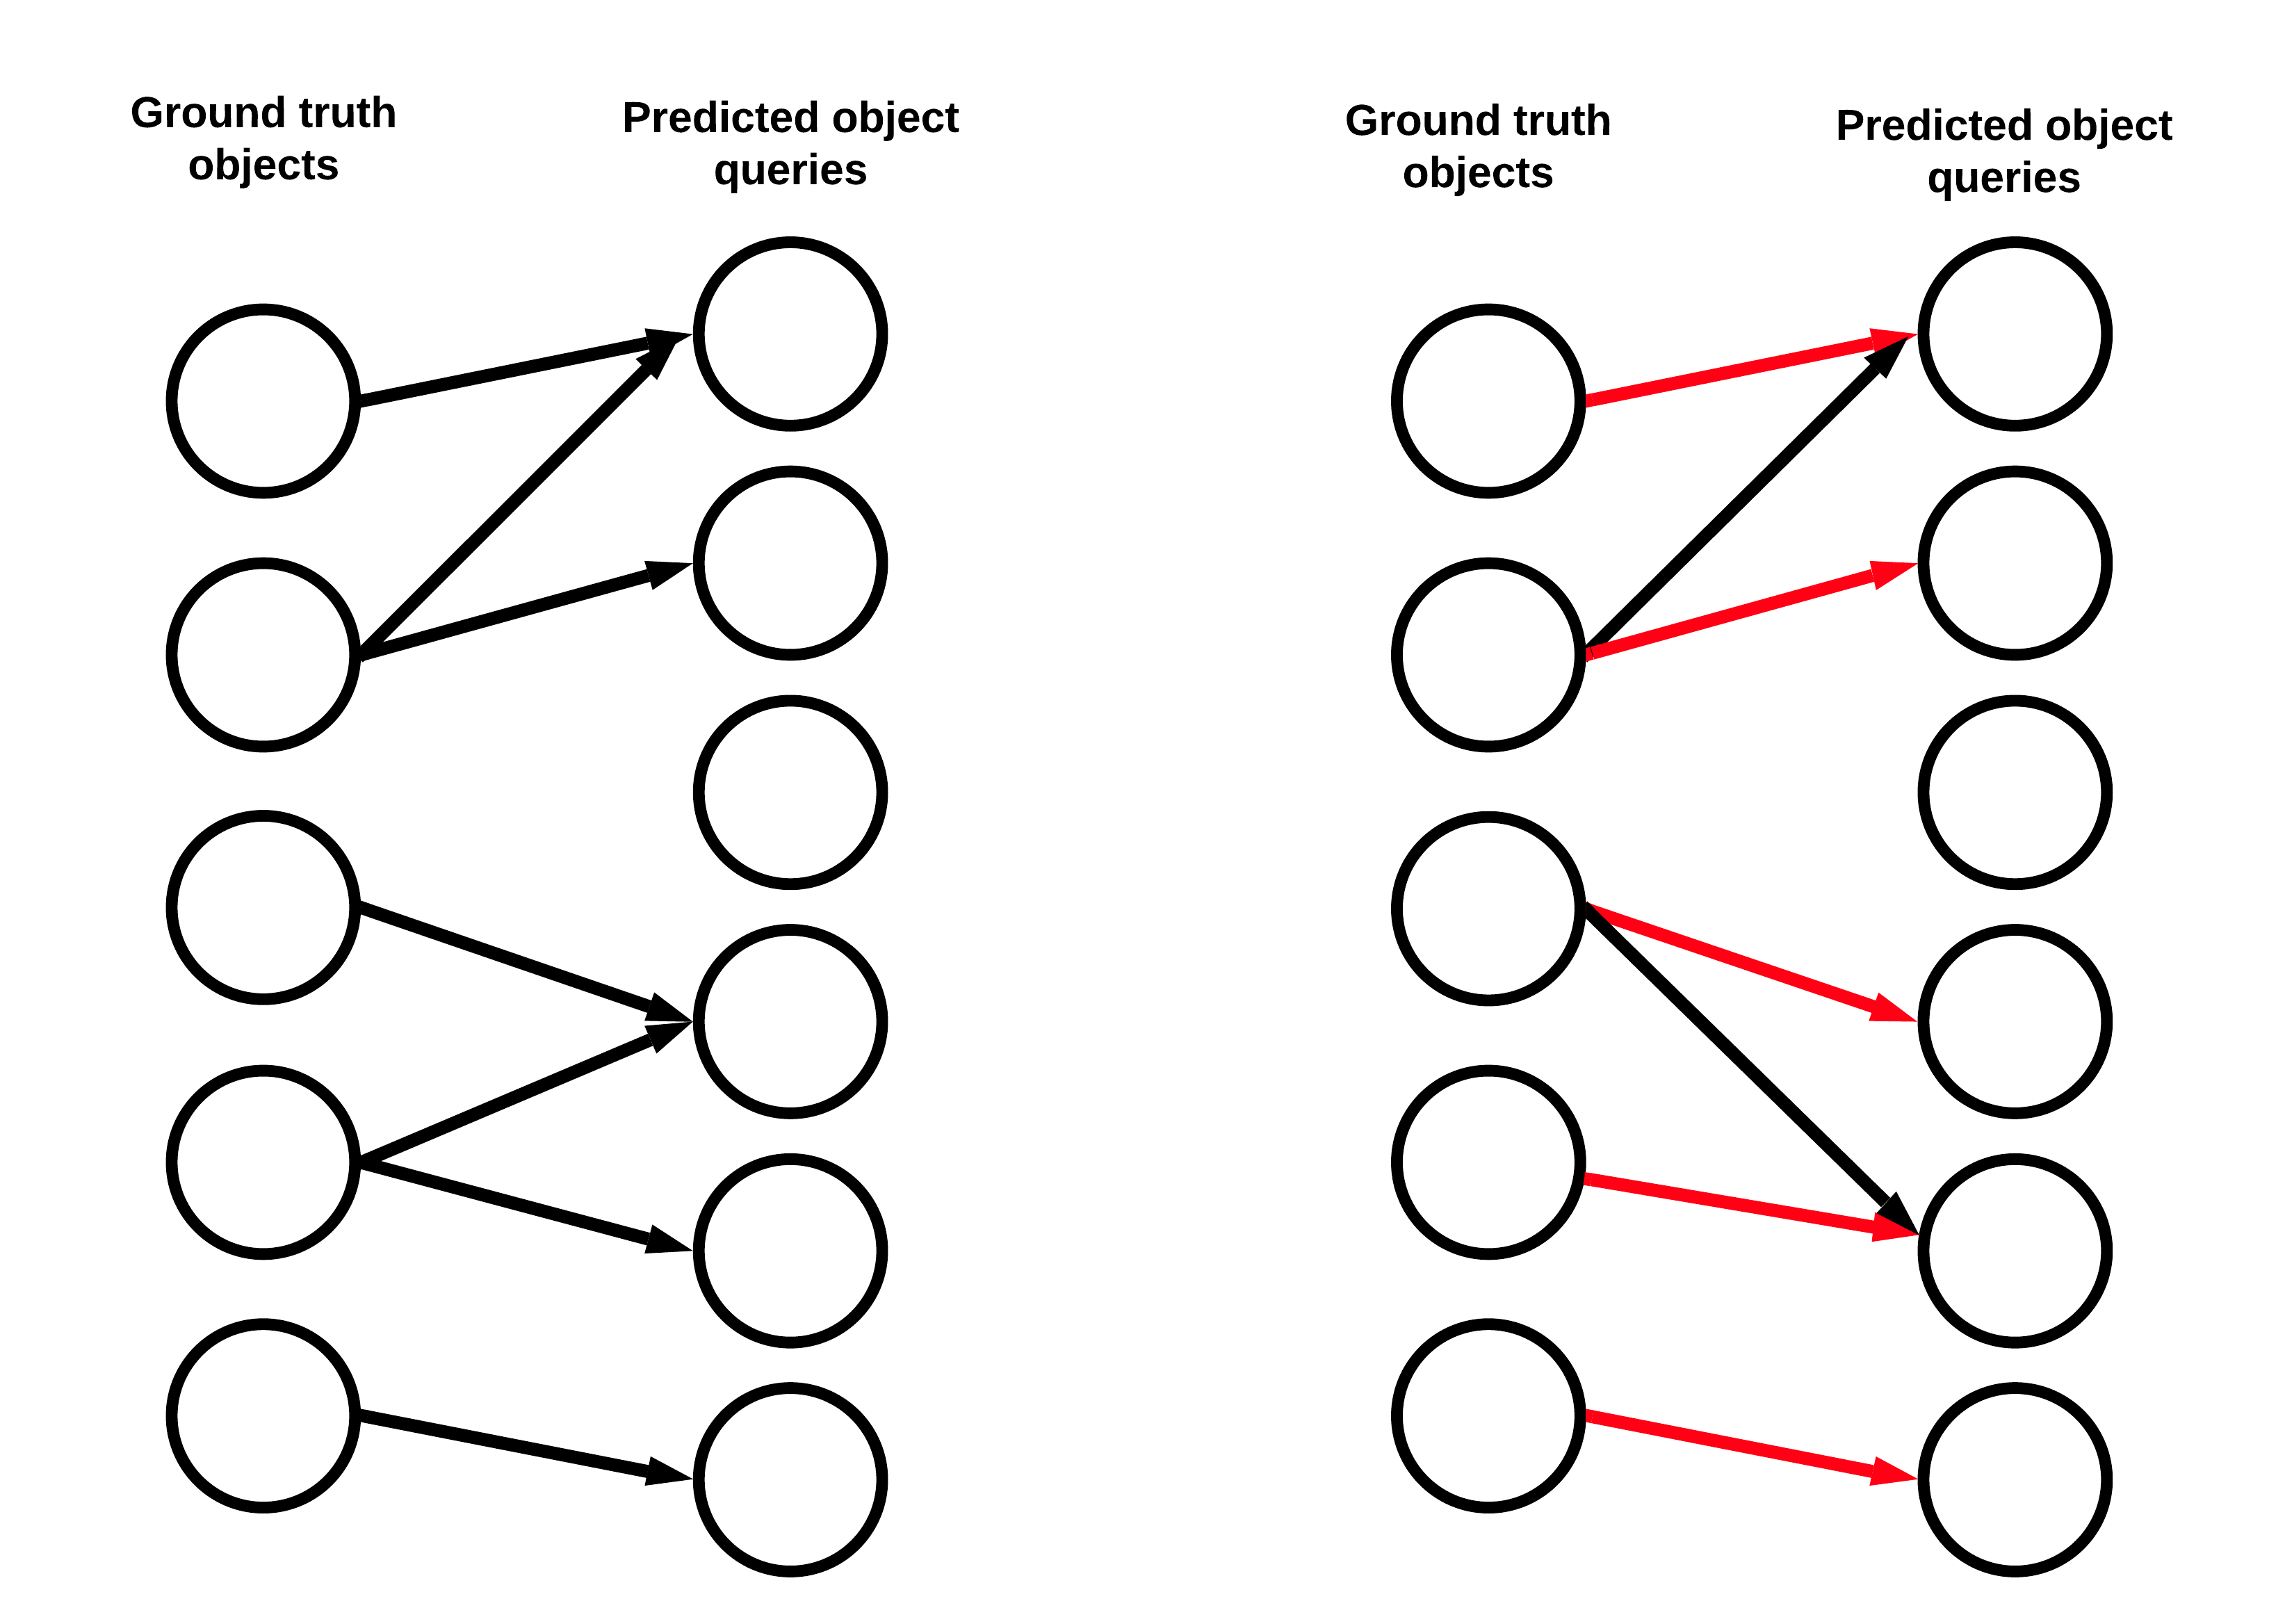
\includegraphics[width=0.8\linewidth]{images/bipartitematching.png}
	\caption{A matching in a bipartite graph. It consists in a set of the edges chosen in such a way that no two edges share an endpoint. The loss function $\hat \sigma$ finds the best match with low cost between the predicted bounding boxes and the ground truth objects.}
	\label{}
\end{figure}

Let $y$ be the ground truth set of objects, and $\hat y = \{\hat y_i\}^{N}_{i = 1}$ the set of $N$ predictions. The bipartite matching between these two sets is a permutation $\hat \sigma$ of $N$ elements $\sigma \in \mathcal{G}_N$ with the lowest cost:

\begin{equation}
\label{formula:bipartitematching}
\hat \sigma = \argmin_{\sigma \in \mathcal{G}_N} \sum_{i}^{N} \mathcal{L}_{match}(y_i, \hat y_{\sigma(i)}),
\end{equation}

where $\mathcal{L}_{match}(y_i, \hat y_{\sigma(i)})$ is a pair-wise \textit{matching cost} between ground truth $y_i$ and a prediction with index $\sigma(i)$. This optimal assignment is computed efficiently
with the Hungarian algorithm \cite{hungarian}. The matching cost taking into account both the class prediction and the similarity between predicted nand ground truth bounding boxes. Each element $i$ can be seen as $y_i = (c_i
, b_i)$ where $c_i$
is the target class label (which may be $\varnothing$) and $b_i \in [0, 1]^{4}$
is a vector that defines ground truth box coordinates and dimensions. For the
prediction with index $\sigma(i)$, the probability of class $c_i$ is defined as $ \hat p_{\sigma(i)}(c_i)$ and
the predicted box as $\hat b_\sigma(i)$. Whit this notations, the authors defines the matching cost as

\begin{equation}
	\mathcal{L}_{match}(y_i, \hat y_{\sigma(i)}) = -\mathds{1}_{\{c \neq \varnothing\}}\hat p_{\sigma(i)}(c_i) + \mathds{1}_{\{c \neq \varnothing\}}\mathcal{L}_{box}(b_i, \hat b_{\sigma(i)}),
\end{equation}
which performs one-to-one matching for direct set prediction without duplicates. The next step is to compute the loss function, called \textit{Hungarian loss}, for all pairs matched in the previous step. It is a linear combination of a negative log-likelihood for class prediction and a box loss defined later:

\begin{equation}
\mathcal{L}_{\text{Hungarian}}(y, \hat y) = \sum_{i = 1}^{N} \bigg [-\log \hat p_{\hat\sigma(i)}(c_i) + \mathds{1}_{\{c \neq \varnothing\}}\mathcal{L}_{box}(b_i, \hat b_{\hat\sigma(i)}) \bigg ]
\end{equation}
where $\hat \sigma$ is the optimal assignment computed in Eq. \ref{formula:bipartitematching}. In practice, the authors
down-weight the log-probability term when $c_i = \varnothing$ by a factor 10 to account for class imbalance. 

\paragraph{Bounding Box Loss} The second part of the matching cost and the Hungarian loss is $\mathcal{L}_{box}(\cdot, \cdot)$ that scores the bounding boxes. The authors makes box predictions directly without some initial guesses using the $\ell_1$ loss. In our context, this loss measures the distance between the ground truth bounding box ($b_i$) and the best predicted box ($\hat b_{\sigma(i)}$) through the L1 norm:

\begin{equation}
\ell_1(b_i - \hat b_{\sigma(i)}) = ||b_i - \hat b_{\sigma(i)}||_1.
\end{equation}

While such approach simplify the implementation, the $\ell_1$ loss will have different scales for small and large boxes even if their relative errors are similar. To mitigate this issue, the final $\mathcal{L}_{box}(\cdot, \cdot)$ is a linear combination of the $\ell_1$ loss and the generalized IoU loss \cite{generalizediou} $\mathcal{L}_{iou}(\cdot, \cdot)$, that is scale invariant. The final bounding box loss is:

\begin{equation}
\mathcal{L}_{box}(b_i, \hat b_{\sigma(i)}) = \lambda_{iou}\mathcal{L}_{iou}(b_i, \hat b_{\sigma(i)}) + \lambda_{L1}||b_i - \hat b_{\sigma(i)}||_1,
\end{equation}
where $\lambda_{iou}$ and $\lambda_{L1}$ are hyper-parameters.

\section{The Simulation Environment}

In this section, it is described the method we propose to build the doors dataset. As mentioned in Sec. \ref{sec:importanceofsimulation}, efficiently collecting a large and heterogeneous visual dataset in the real-world is extremely expensive and time-consuming. The images should be captured from different point of views and illumination conditions to emulate the freedom of movement that characterizes an autonomous agent. Furthermore, the collection procedure must be performed in a large numbers of different scenes and building types, to well generalize the problem. The visual aspect of indoor environments changes a lot according to the building type, the internal design, and the furniture's position.

Following this requirements, we use simulation to compose the visual dataset used in this thesis. As anticipated in Sec. \ref{sec:solution}, we use Gibson \cite{gibson} as simulation environment and Matterport3D \cite{matterport} as worlds dataset. We describe these packages in the following sub-sections.

\subsection{Gibson Environment}

In \citeyear{gibson}, \citeauthor{gibson} published a robotic simulation environment called Gibson \cite{gibson}. Gibson offers real-world perception mechanism for active agents. By perceptual active agent, the authors refer to a
an agent that receives a visual observation from the environment and accordingly effectuates a set of actions, such as locomotion or manipulation. A key question is \textit{where} this sensory observation should come from. Conventional Computer Vision dataset \cite{coco, imagenet} are static and passive, so not suitable for this purpose.  Similarly, learning in the physical world, is not the ideal scenario: the learning speed is extremely slow and the robots are often costly and fragile. Simulation can be solution to mitigate these issues. 
The primary problems around this option are naturally around \textit{generalization
from simulation to real-world}: how to ensure
\begin{enumerate}
	\item \label{enum:generalizationtorealworld1} the semantic
	complexity of the simulated environment is comparable with the real-word, and
	\item \label{enum:generalizationtorealworld2} the rendered frames in simulation are closed enough to the images captured by a camera in the real world (photorealism).
\end{enumerate} 
The main goal of Gibson is to facilitate transferring the
models trained therein to real-world. To overcame the first issue, Gibson offers a frameworks to virtualize environments scanned from the real world and simulates real agents that can interact with the virtual scene. The agent is subject to constraints of space and physics (e.g. collision, gravity). In addition, Gibson implements a mechanism to dissolve differences between virtual renderings and what a real camera would produce (this mitigate the second problem). A neural networks trained to fill the perceptual gap between rendered and real frames.

Gibson’s underlying database of spaces includes 572 full buildings composed of 1447 floors covering a total area of 211k $m^{2}$. Each space has a set of RGB panoramas with global camera poses and reconstructed 3D meshes. To include semantically annotated worlds, the authors also integrated 2D-3D-Semantic dataset \cite{stanford2d3d} and Matterport3D \cite{matterport} (used in this thesis) for easy use.

The Gibson's rendering engine takes a sparse set of RGB-D panoramas in the input and renders a new panorama from an arbitrary novel viewpoint. A ``view'' is a 6D camera pose of $x, y, z$ Cartesian coordinates and roll, pitch, yaw angles, denoted as $\theta, \phi, \gamma$. 

\begin{figure}[h!]
	\centering
	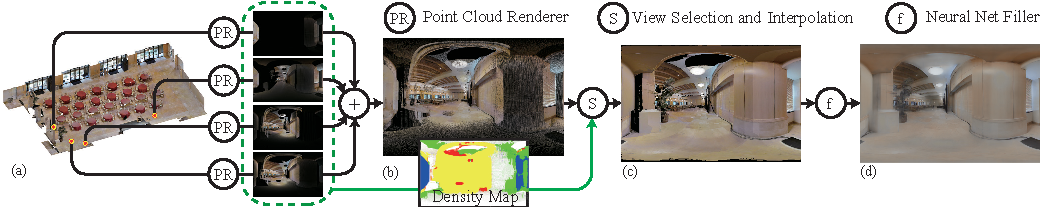
\includegraphics[width=\linewidth]{images/gibson_rendering_pipeline.pdf}
	\caption{The Gibson's rendering pipeline. Image from \cite{gibson}.}
	\label{fig:gibsonrenderingpipeline}
\end{figure}
At first, the given RGB-D panoramas are transformed into point clouds and each pixel is projected from equirectangular coordinates to Cartesian coordinates. For the desired target view $v_j =
(x_j , y_j , z_j , \theta_j, \phi_j, \gamma_j )$, there are chosen the nearest $k$ views in the
scene database, denoted as $v_{j,1}, v_{j,2}, ..., v_{j,k}$, are chosen. The point cloud of each $v_{j,i}$ coordinate are transformed to $v_j$ coordinate with a rigid body transformation and the final point cloud are projected onto an equirectangular image (Fig. \ref{fig:gibsonrenderingpipeline}a). Then, the points from all reference panoramas are aggregated to make a single panorama using a locally weighted mixture (Fig. \ref{fig:gibsonrenderingpipeline}b). To do this, the proposed approach calculates the point density for each spatial position (average number of points per pixel) of each panorama. Hence, the points in the aggregated panorama are adaptively selected from all views. Next, the authors performs a bilinear interpolation on the aggregated points of the final panorama
points in one equirectangular image to reduce the empty space between rendered pixels (Fig. \ref{fig:gibsonrenderingpipeline}c). Finally, the method uses a neural network, called $f$ or ``filler'', to fix artifacts and generate a more real looking image given the output of geometric point cloud rendering (Fig. \ref{fig:gibsonrenderingpipeline}d). This deep model trains a network for making rendered frames look more like real images (forward function) as well as another network which makes real images look like renderings (backward function). The two functions are trained to produce equal outputs. The backward function resembles deployment-time corrective
glasses for the agent, so the authors call it \textit{Goggles}.

\subsection{Matterport3D}






